
\subsection{简介}

\hr

树状数组和下面的线段树可是亲兄弟了,但他俩毕竟还有一些区别:  

树状数组能有的操作,线段树一定有;  

线段树有的操作,树状数组不一定有。

这么看来选择线段树不就\textbf{「得天下了」}?

事实上,树状数组的代码要比线段树短得多,思维也更清晰,在解决一些单点修改的问题时,树状数组是不二之选。

\hr

\subsection{原理}

如果要具体了解树状数组的工作原理,请看下面这张图:

\begin{figure}[htbp]
\centering
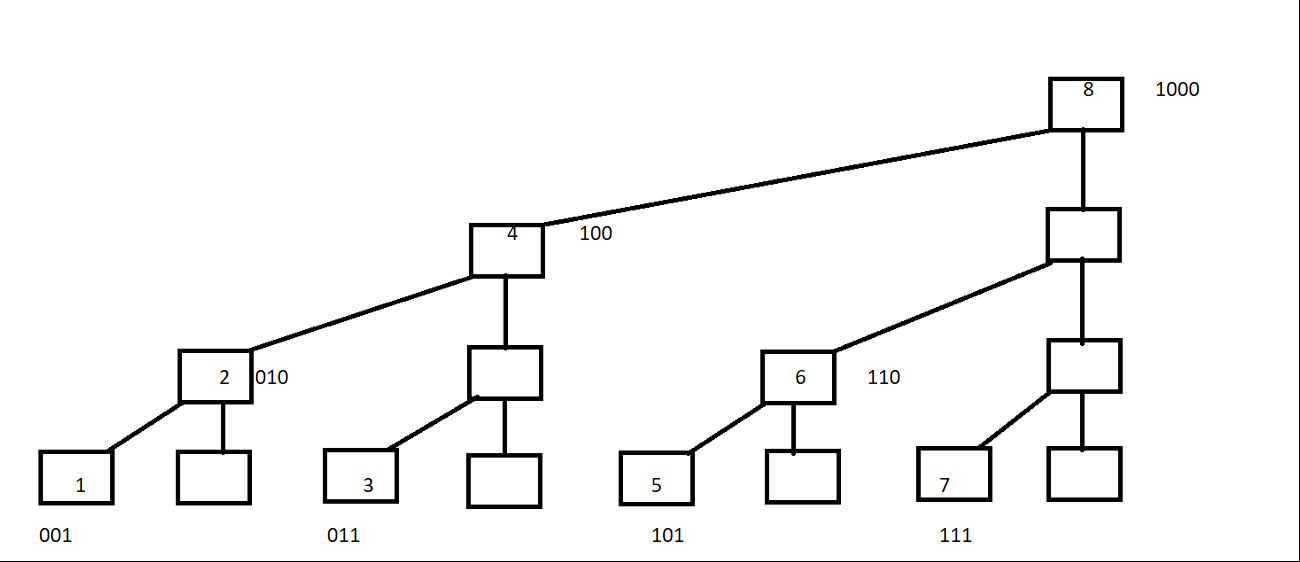
\includegraphics[width=0.7\textwidth]{docs/ds/images/bit1.png} 

\end{figure}

最下面的八个方块就代表存入 $a$ 中的八个数,现在都是十进制。

他们上面的参差不齐的剩下的方块就代表 $a$ 的上级——$c$ 数组。

很显然看出:  

$c[2]$ 管理的是 $a[1]$ \& $a[2]$ ;  

$c[4]$ 管理的是 $a[1]$ \& $a[2]$ \& $a[3]$ \& $a[4]$ ;  

$c[6]$ 管理的是 $a[5]$ \& $a[6]$ ;$c[8]$ 则管理全部 $8$ 个数。

所以,如果你要算区间和的话,比如说要算 $a[51]$ \textasciitilde{} $a[91]$ 的区间和,暴力算当然可以,那上百万的数,那就 RE 喽。

那么这种类似于跳一跳的连续跳到中心点而分值不断变大的原理是一样的(倍增)。

你从 $91$ 开始往前跳,发现 $c[n]$($n$ 我也不确定是多少,算起来太麻烦,就意思一下)只管 $a[91]$ 这个点,那么你就会找 $a[90]$,发现 $c[n - 1]$ 管的是 $a[90]$ \& $a[89]$ ;那么你就会直接跳到 $a[88]$ ,$c[n - 2]$ 就会管 $a[81]$ \textasciitilde{} $a[88]$ 这些数,下次查询从 $a[80]$ 往前找,以此类推。

\hr

\subsection{用法及操作}

那么问题来了,你是怎么知道 $c$ 管的 $a$ 的个数分别是多少呢?你那个 $1$ 个,$2$ 个,$8$ 个…… 是怎么来的呢?

这时,我们引入一个函数—— \texttt{lowbit}:

\begin{cppcode}
int lowbit(int x) {
  //算出x二进制的从右往左出现第一个1以及这个1之后的那些0组成数的二进制对应的十进制的数
  return x & -x;
}
\end{cppcode}

\texttt{lowbit} 的意思注释说明了,咱们就用这个说法来证明一下 $a[88]$:  

$88_{(10)}=1011000_{(2)}$  

发现第一个 $1$ 以及他后面的 $0$ 组成的二进制是 $1000$  

$1000_{(2)} = 8_{(10)}$  

$1000$ 对应的十进制是 $8$,所以 $c$ 一共管理 $8$ 个 $a$。

这就是 \texttt{lowbit} 的用处,仅此而已(但也相当有用)。

\textbf{你可能又问了:x \& -x 是什么意思啊?}

\begin{QUOTE}{}{}
$-x$ 代表 $x$ 的负数,计算机中负数使用对应的正数的补码来表示。
\end{QUOTE}

例如 :  

$x =88_{(10)}=1011000_{(2)}$;  

$-x = -88_{(10)} = (0100111_{(2)} + 1_{(2)}) =101000_{(2)}$;  

$x\ \& \ (-x) = 1000_{(2)} = 8_{(10)}$。

神奇吧,我也觉得神奇!

那么对于\textbf{单点修改}就更轻松了:

\begin{cppcode}
void change(int x, int k) {
  while (x <= n)  //不能越界
  {
    c[x] = c[x] + k;
    x = x + lowbit(x);
  }
}
\end{cppcode}

每次只要在他的上级那里更新就行,自己就可以不用管了。

\begin{cppcode}
int getsum(int x)  // a[1]……a[x]的和
{
  int ans = 0;
  while (x >= 1) {
    ans = ans + c[x];
    x = x - lowbit(x);
  }
  return ans;
}
\end{cppcode}

\textbf{区间和}也不用说了吧,代码十分清真。

\subsection{例题}

\href{https://www.luogu.org/problemnew/show/P3374}{传送门}  

\href{https://www.luogu.org/problemnew/show/P3368}{传送门 2}
